\section[F. de hash y autentificación en la práctica]{Funciones de hash y autentificación en la práctica}
Una función de hash se construye de la siguiente manera:
\begin{itemize}
    \item Se define una función de hash para mensajes de largo fijo, la cual es llamada \textbf{función de compresión}.
    \item Se define un método que permite utilizar de manera \textbf{iterativa} la función de compresión para construir una función de hash para mensajes de \textbf{largo arbitrario}.
\end{itemize}

Por ejemplo, digamos que queremos construir una función de hash de largo fijo (de compresión) tal que:
$$
h:\{0,1\}^{2n} \to \{0,1\}^n
$$
Para la construcción supondremos que tenemos un esquema criptográfico $(\gen, \enc, \dec)$ sobre los espacios $\ca{M} = \ca{K} = \ca{C} = \{0,1\}^n$, donde:
$$
\enc_k:\{0,1\}^n \to \{0,1\}^n \quad \text{para cada } k \in \{0,1\}^n
$$
En un primer intento, podemos definir, dados $u,v \in \{0,1\}^n,$ la función $h(u||v) = \enc_u(v)$, es decir, nuestra función de hash encripta $v$ usando a $u$ como llave. El problema de esta implementación es que existe un algoritmo eficiente, en términos del parámetro de seguridad $1^n$, que puede construir preimágenes de esta función $h$. \medbreak

En términos más generales, fijemos una llave $k \in \{0,1\}^n$ y definamos las siguientes funciones de $\{0,1\}^n$ a $\{0,1\}^n$:
$$
f(x) = \enc_k(x) \qquad g(x) = \dec_k(x)
$$
Ya hemos demostrado anteriormente que $\forall x \in \{0,1\}^n: g(f(x)) = x$, pero, ¿se cumple también $f(g(x)) = x$? Esto depende del conjunto en el que se muevan las funciones $f$ y $g$, por ejemplo:
\img{img/cap5/1.png}{0.45}

Si hay alguna preimagen con dos preimágenes, no se cumple siempre que $f(g(x)) = x$, puesto que podríamos llegar a dos valores diferentes para $x$. Sin embargo, si nos encontramos en el caso en que $\ca{M} = \ca{C} = \{0,1\}^n$, tenemos que:
$$
\forall x \in \{0,1\}^n: f(g(x)) = x
$$
y por ende podemos concluir que:
$$
\forall k \in \ca{K}.\,\forall m \in \ca{M}: \enc_k(\dec_k(m)) = m
$$
Con lo anterior, podemos demostrar que nuestro primer intento de función de hash no es resistente a preimagen. Consideremos $u' \in \{0,1\}^n$ arbitrario, y definimos $v' = \dec_{u'}(x)$. Tenemos entonces que
$$
h(u'||v') = \enc_{u'}(v') = \enc_{u'}(\dec_{u'}(x)) = x
$$
Necesitamos una construcción mejor para funciones de hash.

\subsection{Construcción de Davies-Meyer}
La función de hash de Davies-Meyer se define como:
\alignformula{
    h(u||v) = \enc_u(v) \oplus v
}

Recordando que $\oplus$ representa la operación XOR, o en el caso de trabajar con bits, la suma en módulo 2.

\paragraph{Formalización.} Sea un esquema criptográfico $(\gen, \enc, \dec)$ definido sobre los espacios $\ca{M} = \ca{K} = \ca{C} = \{0,1\}^*$. Definimos una función de hash $(\gen', h')$ de largo fijo tal que:
\begin{itemize}
    \item $\gen'(1^n) = n$ para un parámetro de seguridad $1^n$.
    \item $(h')^n:\{0,1\}^{2n} \to \{0,1\}^n$ tal que para cada $u,v \in \{0,1\}^n$:
    $$
    (h')^n(u||v) = \enc_u(v) \oplus v
    $$
\end{itemize}

\paragraph{Propiedad fundamental.} Si $(\gen, \enc, \dec)$ es un esquema criptográfico \textit{ideal}, entonces $(\gen', h')$ es resistente a colisiones. Por ende, $(\gen', h')$ es una buena alternativa para una función de compresión.

\paragraph{Extensión a largo arbitrario.} Suponemos que tenemos una función de compresión $h':\{0,1\}^{256} \to \{0,1\}^{128}$ y un mensaje $m$ de largo arbitrario. Podemos dividir el mensaje en bloques de 128 bits e ir aplicando la función de hash de la siguiente manera:
\img{img/cap5/2.png}{0.4}
\img{img/cap5/3.png}{0.4}
$H_0$ es un \textbf{vector de inicialización} de la función de hash, y se define de manera previa. Para analizar la intuición de esta idea, es posible demostrar que si $h'$ es resistente a colisiones, y no se conoce una preimagen de $H_0$, entonces $h$ es resistente a colisiones. La idea de esta demostración se vuelve más sencilla en el caso de mensajes cuyo largo es divisible por 128, y donde los mensajes en una colisión tienen el mismo largo. Esta demostración queda propuesta para el lector.

\paragraph{El vector de inicialización $H_0$.} ¿Podríamos pedir que $H_0$ sea un número sacado al azar? Esto es peligroso ya que un adversario puede sacar un mensaje $m_0 \in \{0,1\}^{256}$ y decir que $H_0 = h'(m_0)$. Este $H_0$ se ve como un número sacado al azar, pero el adversario conoce una preimagen, que es $m_0$. \medbreak

Entonces, ¿cómo podemos estar seguros de que nadie conoce una preimagen de $H_0$? Lo que necesitamos es un \textbf{nothing-up-my-sleeve number}, es decir, un número que ha sido escogido de tal manera que evita la posibilidad de que alguien pueda argumentar que el número ha sido seleccionado con una intención oculta de manipular el sistema. Estos números ayudan a demostrar que no hay ``trucos ocultos'' en la elección de estas constantes, es decir, no hay nada escondido bajo la manga. Un ejemplo podría ser los primeros 128 bits de la representación de $\pi$ en binario, ¿alguien podría conocer una preimagen de este valor de $H_0$?

\paragraph{Padding.} En el caso en que los mensajes no sean divisibles por un valor $n$, debemos hacer \textbf{padding}, por ejemplo, agregar 0's al final del mensaje:
\begin{figure}[H]
\centering
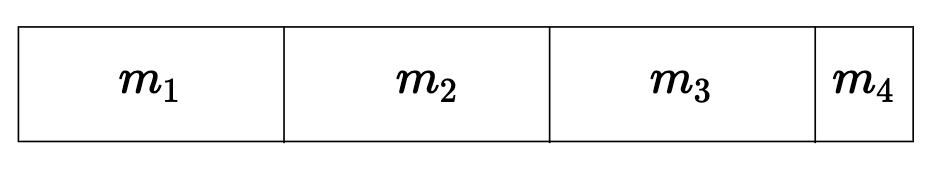
\includegraphics[scale=0.4]{img/cap5/4.png}
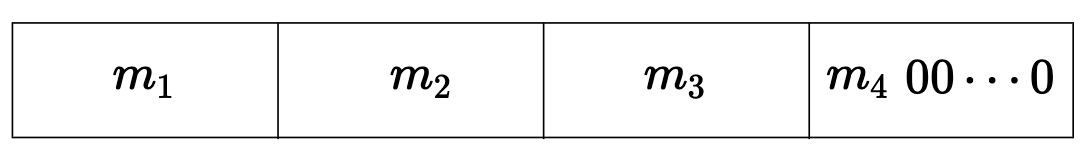
\includegraphics[scale=0.4]{img/cap5/5.png}
\end{figure}

Sin embargo, esta no es una buena idea ya que es fácil encontrar colisiones: $h(m) = h(m0)$ si $|m|$ no es divisible por 128. Entonces, ¿qué debe cumplir una buena función de padding? Consideremos una función $Pad(\cdot)$ para bloques de largo $n$, por ejemplo, $n = 128$. Dado un mensaje $m \in \{0,1\}^*$, se debe tener que
$$
|Pad(m)| \geq n \quad \text{y} |Pad(m)| \quad \text{ es divisible por } n
$$
Los axiomas fundamentales del padding son:
\begin{itemize}
    \item $m$ es un prefijo de $Pad(m)$.
    \item si $|m_1| = |m_2|$, entonces $|Pad(m_1)| = |Pad(m_2)|$.
    \item si $|m_1| \neq |m_2|$, entonces el último bloque de $Pad(m_1)$ es distinto del último bloque de $Pad(m_2)$/
\end{itemize}
Si un padding cumple con estos axiomas, entonces $Pad$ es una \textbf{función inyectiva}. Si suponemos que $m_1 \neq m_2$, entonces:
\begin{itemize}
    \item si $|m_1| \neq |m_2|$, entonces $Pad(m_1) \neq Pad(m_2)$ ya que el último bloque de $Pad(m_1)$ es distinto del último bloque de $Pad(m_2)$.
    \item si $|m_1| = |m_2|$, entonces $Pad(m_1) \neq Pad(m_2)$ ya que $m_1$ es prefijo de $Pad(m_1)$ y $m_2$ es prefijo de $Pad(m_2)$.
\end{itemize}

\subsection{Construcción de Merkle-Damgård}
Juntando todo lo anterior, supongamos dados:
\begin{itemize}
    \item La función de compresión $(\gen, h')$ de Davies-Meyer.
    \item Para cada $n \in \mathbb{N}$, una función de padding $Pad_n$, que considera bloques con $n$ elementos y satisface los axiomas fundamentales.
\end{itemize}
Vamos a definir una función de hash $(\gen, h)$ para mensajes de largo arbitrario. Consideremos un parámetro de seguridad $1^n$, entonces, tenemos que $\gen(1^n) = s$ y luego $h^s:\{0,1\}^* \to \{0,1\}^n$. \medbreak

El valor del vector de inicialización $H_0$ está contenido en $s$, ya que $s$ puede ser definido como $(n, H_0)$. Luego, dado un $m \in \{0,1\}^*$, calculamos $h^s(m)$ de la siguiente forma:
\begin{enumerate}
    \item Supongamos que $Pad_n(m) = m_1 m_2 \cdots m_\ell$, donde el largo de cada bloque $m_i$ es $n$.
    \item Para cada $i \in \{1, \ldots, \ell\}$: $H_i = (h')^n(m_1 || H_{i-1})$
    \item $h^s(m) = H_\ell$
\end{enumerate}

Esta construcción $(\gen, h)$ es resistente a colisiones. Queda como ejercicio propuesto al lector demostrar esta afirmación, dado que $(\gen', h')$ es resistente a colsiones y cada función de padding $Pad_n$ satisface los axiomas fundamentales. Notar que:
\begin{itemize}
    \item Podemos reemplazar la construcción de Davies-Meyer por cualquier función de compresión resistente a colisiones.
    \item Podemos considerar funciones de compresión de la forma $h':\{0,1\}^{p(n)} \to \{0,1\}^n$, con $p(n)$ un polinomio tal que $p(n) > n$.
\end{itemize}

Pero, ¿qué función de padding usamos? Consideramos bloques de largo $n$:
\begin{figure}[H]
    \centering
    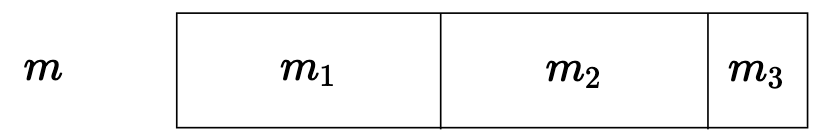
\includegraphics[scale=0.35]{img/cap5/6.png}
    \hspace{1.51cm}
    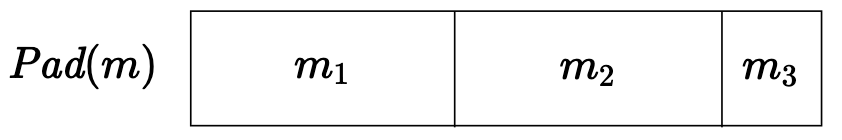
\includegraphics[scale=0.35]{img/cap5/7.png}
    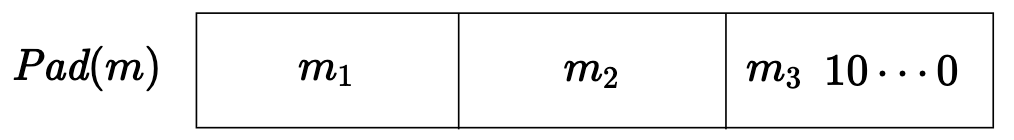
\includegraphics[scale=0.35]{img/cap5/8.png}
    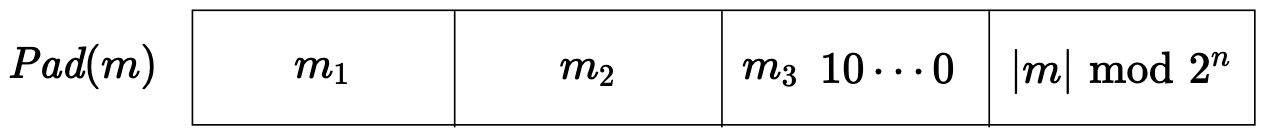
\includegraphics[scale=0.35]{img/cap5/9.png}
\end{figure}

Esta función de padding satisface los dos primeros axiomas fundamentales, pero pueden existir mensajes $m_1$ y $m_2$ tales que $|m_1| \neq |m_2|$ y los últimos bloques de $m_1$ y $m_2$ son iguales. Se debe tener que: $|m_1| \equiv |m_2| \bmod 2^n$, ya que si $|m_1| < |m_2|$, entonces $|m_2| > 2^n$. \medbreak

Si $n = 128$, entonces $|m_2| > 2^{128}$, y $m_2$ debe tener al menos $10^{38}$ dígitos. ¿Es posible escribir un número de este tamaño? \textbf{No.} Cisco estima que el tráfico de Internet en 2025 será de 175 zettabytes, vale decir, $175 \cdot 10^{21}$ bytes.

\subsection{Secure Hash Algorithm 2 (SHA-2)}
SHA-2 es una familia de funciones de funciones de hash.
\begin{itemize}
    \item Se definen utilizando la construcción de Merkle-Damgård
    \item Las funcoines de compresión son definidas utilizando la construcción de Davies-Meyer sobre un block cipher propio (no el de AES).
\end{itemize}
Por ejemplo, en SHA-256, el número se refiere al largo del hash. Esta función es una función de $\{0,1\}^*$ a $\{0,1\}^{256}$. SHA-256 puede considerarse como el resultado de instanciar el parámetro de seguridad el el valor 256 (de hecho, se usa en Bitcoin). También son utilizados otros ejemplos como SHA-224, SHA-384 y SHA-512. 

\paragraph{SHA-256.} Considera bloques de 512 bits, y sus estados internos $H_i$ son de 256 bits. La función de compresión es de la forma:
$$
h':\{0,1\}^{512} \times \{0,1\}^{256} \to \{0,1\}^{256}
$$
La función de padding se define utilizando las ideas descritas en las secciones anteriores, pero reservando los últimos 64 bits para el largo del mensaje $m$. Se realizan los siguientes pasos sobre el mensaje $m$:
\begin{enumerate}
    \item Se agrega un símbolo 1.
    \item Se agregan $\ell$ símbolos 0, donde $\ell$ es el menor número natural tal que $|m| + 1 + \ell \equiv 448 \bmod 512$.
    \item Se agrega $|m| \bmod 2^{64}$.
\end{enumerate}
El vector de inicialización $H_0$ se define como $H_0^1H_0^2H_0^3H_0^4H_0^51H_0^61H_0^7H_0^8$, donde $H_0^i$ tiene los primeros 32 bits de la parte decimal de la raíz cuadrada del $i$-ésimo número primo. Por ejemplo, $H_0^1$ tiene los primeros 32 bits de la parte decimal de $\sqrt{2}$:
$$
H_0^1 = 01101010000010011110011001100111
$$

\subsection{HMAC}
HMAC, siglas en inglés correspondientes a \textit{Hash-based message authentication code}, corresponde a la construcción de un código de autentificación de mensajes $\mac$ en base a una función de hash $h$. ¿Qué pasa si definimos $\mac_k(m) = h(k || m)$? Recordemos el juego que definía un buen MAC:
\begin{enumerate}
    \item El verificador genera una llave $k$.
    \item El adversario envía $m_0 \in \ca{M}$.
    \item El verificador responde $\mac_k(m_0)$.
    \item Los pasos 2 y 3 se repiten tantas veces como quiera el adversario.
    \item El adversario envía $(m,t)$, siendo $m$ un mensaje que no se había enviado antes.
\end{enumerate}
El adversario gana si $\ver_k(m,t) = 1$. Ahora, pensemos que estamos usando SHA-2, ¿puede el adversario ganar el juego? Hagamos una simplificación, el largo de $k$ es un bloque:
\img{img/cap5/10.png}{0.4}
Donde:
\begin{itemize}
    \item $k \, m_0 \cdots m_\ell$ es en realidad $Pad(k||m)$.
    \item En particular, $m \neq m_0 \cdots m_\ell$. 
\end{itemize}
Entonces, ¿cómo se ve $Pad(Pad(k||m))$?
$$
Pad(Pad(k||m)) = k\,m_0 \cdots m_\ell \, m_{\ell + 1}
$$
Por lo tanto, el adversario puede calcular y ganar el juego:
\img{img/cap5/11.png}{0.4}

Donde $m' = m_0 \cdots m_\ell$. Este tipo de ataques se conoce como \textit{length extension attacks}. \medbreak

Si tratamos con $\mac_k(m) = h(m||k)$ (al revés del ejemplo anterior), no podemos hacer ataques de extensión de largo, pero si puede ocurrir una colisión de dos mensajes del mismo largo, que termina rompiendo el MAC.
\img{img/cap5/12.png}{0.4}

Podemos seguir tratando varias funciones de hash, pero lo que podemos \textit{intuir} que es seguro es
$$
\mac_k(m) = h(k_2 \mid\mid h(k_1 \mid\mid m))
$$
donde $k_1$ y $k_2$ ocupan exclusivamente un bloque, son distintas, se derivan de forma determinista a partir de $k$ y no se pueden obtener sin $k$. El estándar se define de la siguiente forma:
$$
k' = \begin{cases}
h(k) &k\text{ usa más de un bloque} \\
k &\text{e.o.c.}
\end{cases}
$$
Así, podemos definir a $\hmac$ como:
$$
\hmac_k(m) = h(k_2 \mid\mid h(k_1 \mid\mid m))
$$
\img{img/cap5/13.png}{0.4}
